
\chapter{Introducci\'on}\label{capit:cap1}
\vspace{-2.0325ex}%
\noindent
\rule{\textwidth}{0.5pt}
\vspace{-5.5ex}% 
\newcommand{\pushline}{\Indp}

Aqu\'i la introducci\'on pls
\section{Antecendentes}
Antecedentes aqui pls
\section{Plantamiento del problema}
	La demencia es un s\'indrome del declive de las habilidades cognitivas. Los s\'intomas comunes son: problemas de memoria, dificultades para realizar tareas, mal juicio, deterioro del lenguaje hablado y cambios de humor\citep{Aziz}. Afecta alrededor del 4\% de las personas mayores de 65 a\~nos y al 40\% de las personas mayores de 90.
	        En un estudio, 60\% de los cuidadores desarrollaron un desorden depresivo y/o de ansiedad en los primeros 24 meses: 37\% de depresi\'on, 55\% desorden de ansiedad y 32\% ambos. \citep{Joling2014}. Casi un cuarto de los cuidadores de personas con demencia tienen un nivel de ansiedad cl\'inico significante \citep{Cooper200615}.Mientras que la carga de los cuidadores informales aumenta, se vuelve mas probable que sufran de ansiedad y depresi\'on \citep{Denno20131731}. La carga en los cuidadores (f\'isica o psicol\'ogica) podr\'ia aumentar los niveles de ansiedad. Entre mas demandante es un servicio, mayor podr\'ia ser la ansiedad percibida. Los comportamientos bizarros o impredecibles de la persona afectada por demencia aumentan la carga emocional \citep{Rosa201054}. En este estudio, se har\'a uso del c\'omputo vestible para capturar informaci\'on de ansiedad y se utilizar\'a aprendizaje de m\'aquina para detectar periodos de ansiedad en cuidadores de personas con demencia.

\section{Objectivos}
\subsection{Objetivo general}
	Detectar periodos de ansiedad en cuidadores de personas con demencia por medio de c\'omputo vestible
\subsection{Objetivos espec\'ificos}
\subsection{Hip\'otesis de investigaci\'on}
	Se puede detectar ansiedad usando dispositivos vestibles...
\subsection{Propuesta de la soluci\'on}
	Propuesta del experimento para obtener datos...

\section{Metodolog\'ia}\label{secc:methodology}
La metodolog\'ia seguida se bas\'o en tres pasos: \textit{Captura de datos}, \textit{Detecci\'on de ansiedad}, y un paso hipot\'etico de \textit{Estrategias de afrontamiento} (ver figura ~\ref{fig:metodology}). El primer paso consiste en recabar informaci\'on de cuidadores bajo situaciones de ansiedad con el fin de etiquetar eventos. Esta captura se logr\'o por medio de un experimento que implementa una t\'ecnica de ``Naturalistic Enactment''. Una vez capturada y etiquetada la informaci\'on, se desarroll\'o un m\'etodo basado en t\'ecnicas de aprendizaje de m\'aquina que tom\'o los segmentos de ansiedad y se extrajeron caracter\'isticas personales de cada se\~nal con tal de caracter\'izar dichos eventos. El tercer paso, aunque queda fuera del alcance de esta tesis se discute como las posibles aplicaciones por medio de tecnolog\'ia m\'ovil y/o pantallas ambientales y c\'omo ser\'ia un concepto de aplicaci\'on real. (Ver Trabajo a futuro)
\begin{figure}[h]
        \centering
        \subfigure[]{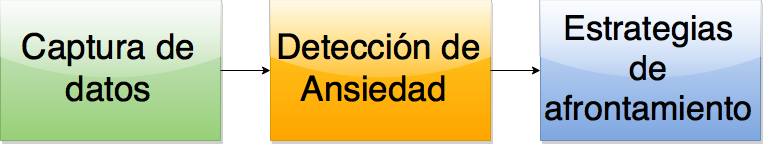
\includegraphics[width=160mm]{./Figures/img_metodologia}}
        \caption{Metodolog\'ia seguida durante la investigaci\'on.} \label{fig:metodology}
\end{figure}
\subsection{Contribuci\'on}
\subsection{Conclusi\'on}
\subsection{Organizaci\'on de la tesis}
\section{Pregunta de investigac\'ion}
	?`C\'omo pueden los dispositivos vestibles ayudar a detectar ansiedad en cuidadores de personas con demencia?
\section{Hip\'otesis}
	\begin{itemize}
	\item{Los sujetos tendr\'an mayores valores en las caracter\'isticas de GSR y EEG durante un periodo de ansiedad alto que durante uno bajo.}
	\item{Los sujetos tendr\'an mayor valor HR promedio durante un periodo de ansiedad alto que durante uno bajo}
	\item{Los sujetos que reporten mayores valores en la prueba de SUDS tendr\'an mayores valores en las caracter\'isticas de GSR, HR, y EEG durante un periodo de ansiedad.}
	\end{itemize}
\section{Variables independientes}
	\begin{itemize}
		\item{Periodos con ansiedad}
		\item{Periodos sin ansiedad}
	\end{itemize}
\section{Variables dependientes}
	\begin{itemize}
		\item{Caracter\'isticas de GSR: N\'umero de picos por segmento, Amplitud y tiempo de recuperaci\'on medio}
		\item{Valor de HR: Promedio de HR}
	\end{itemize}
\section{Escenario}
	Los participantes ser\'an transportados del departamento de computaci\'on de CICESE hacia una casa donde se encontrar\'a el adulto mayor
	para realizar la prueba.
	Se les pedir\'a reposar durante 15 minutos en el lugar para regularizar su sudoraci\'on y ritmo cardiaco.
	Luego, se les tomar\'a una muestra de 5 minutos de sus se\~nales fisiol\'ogicas como l\'inea base por medio de una banda para HR, una pulsera para GSR y una diadema para EEG. Durante estos 5 minutos
	se les pedir\'a  que reposen sentados en una habitaci\'on sin el adulto mayor y con los ojos cerrados, concetr\'andose en su respiraci\'on como t\'ecnica de relajaci\'on.

	Pasado el tiempo de relajaci\'on se les presentar\'a al adulto mayor en una habitaci\'on diferente.Despu\'es de la introducci\'on llevar\'an a cabo la terapia. Una vez mas, llevar\'an sobre el cuerpo la banda de ritmo cardiaco, la pulsera para GSR y la diadema de EEG. Durante la prueba, se les pedir\'a que reporten su nivel de ansiedad por medio de un formato especial (Ver anexo [] )

\section{Configuraci\'on del escenario}
	
	Los datos ser\'an capturados de la siguiente manera:
	\begin{itemize}
		\item{La se\~nal de suduraci\'on se obtendr\'a por medio de la pulsera \textbf{Empatica E3} que ser\'a conectada a un tel\'efono inteligente Samsung S4 con android 4.0 ejecutando la aplicaci\'on CareMeToo hecha en el laboratorio.}
		\item{La se\~nal de ritmo cardiaco se obtendr\'a por medio de una banda zephyr HxM conectado a una macbook 2008 ejecutando la aplicaci\'on \textbf{anxiLogger} hecha en el laboratorio.}
		\item{La se\~nal de EEG se obtendr\'a por medio de la diadema Muse conecatada a la misma macbook 2008 ejecutando la aplicaci\'on Muse Lab.}
		\item{Todo el procedimiento ser\'a grabado por medio de una c\'amara Sony HD instalada en el lugar.}
	\end{itemize}
\section{Consideraciones}
	\begin{itemize}
		\item{Los participantes no podr\'an tomar bebidas con cafe\'ina (caf\'e, t\'e, refresco, bebidas energ\'eticas etc.) durante al menos 8 horas antes de la prueba.}
		\item{Los participantes no podr\'an interactuar con los investigadores una vez que inicie la prueba.}
		\item{El papel del adulto mayor ser\'a realizado por una actriz profesional con experiencia en papeles de adultos mayores y aconsejada en el comportamiento de una persona con demencia por una profesional.}
		\item{Los participantes ser\'an previamente entrenados en la aplicaci\'on de la terapia unos dias antes de la prueba.}
	\end{itemize}
\section{Metodolog\'ia}
	Los eventos ser\'an clasificados como de alta ansiedad y baja ansiedad con ayuda de comportamientos preparados y marcadores en los tiempos con ayuda del video.
	Se segmentar\'an las se\~nales en periodos de tiempo de acuerdo con los marcadores y se realizar\'a un an\'alisis estad\'istico para determinar diferencias significativas y corroborar las etiquetas. Los datos ser\'an procesados con utiler\'ias ya programadas en python. Por \'ultimo se utilizar\'a aprendizaje de m\'aquina para clasificar los eventos.
\newpage
%%=====================================================
